\documentclass[border=6pt]{standalone}
\usepackage{tikz}
\usetikzlibrary{arrows.meta,positioning,fit,calc,backgrounds}
\begin{document}
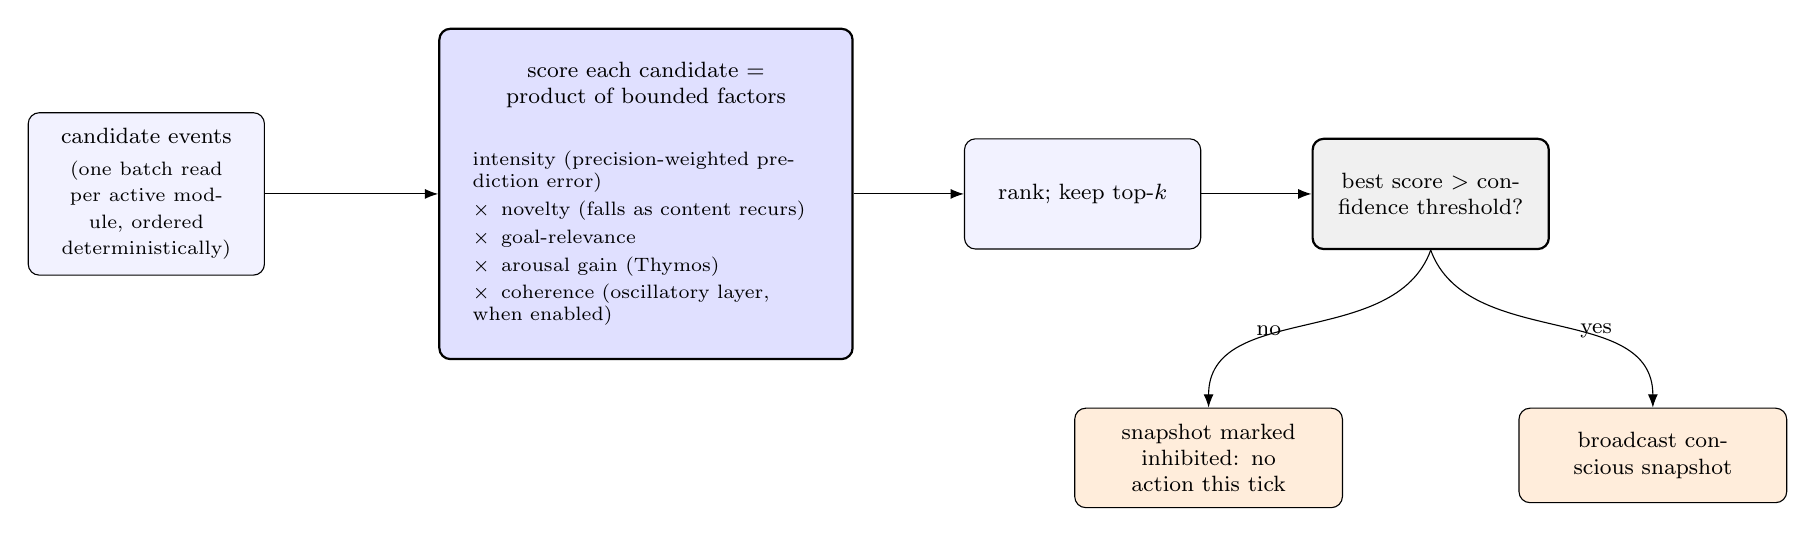
\begin{tikzpicture}[
  font=\small,>=Latex,
  stage/.style={draw, rounded corners, fill=blue!5, align=center, minimum height=14mm, font=\footnotesize, text width=26mm, inner sep=2mm},
  scorebox/.style={draw, thick, rounded corners, fill=blue!12, align=center, minimum height=34mm, font=\footnotesize, text width=48mm, inner sep=2.5mm},
  decide/.style={draw, thick, rounded corners, fill=gray!12, align=center, minimum height=14mm, font=\footnotesize, text width=26mm, inner sep=2mm},
  outbox/.style={draw, rounded corners, fill=orange!14, align=center, minimum height=12mm, font=\footnotesize, text width=30mm, inner sep=2mm},
]

% (b) scoring -- factor list lives inside the box so no arrow ever crosses it.
% Built from two separately-aligned nodes (title centered, list left-aligned)
% and a background-layer fit rectangle, so centering the title cannot stagger
% the left-aligned list underneath it. Placed first, at the origin, so the
% other pipeline stages can be centered on ITS vertical midpoint (not the
% other way around) and every connecting arrow comes out perfectly horizontal.
\node[align=center, font=\footnotesize, text width=44mm] (scoretitle) at (0,0)
  {score each candidate $=$ product of bounded factors};
\node[align=left, font=\scriptsize, text width=44mm, below=3mm of scoretitle] (scorelist)
  {intensity (precision-weighted prediction error)\\[2pt]
   $\times$\, novelty (falls as content recurs)\\[2pt]
   $\times$\, goal-relevance\\[2pt]
   $\times$\, arousal gain (Thymos)\\[2pt]
   $\times$\, coherence (oscillatory layer, when enabled)};
\begin{pgfonlayer}{background}
\node[draw, thick, rounded corners, fill=blue!12, fit=(scoretitle)(scorelist), inner sep=3mm] (score) {};
\end{pgfonlayer}

% (a) candidate events -- centered on the score box's vertical midpoint
\node[stage, left=22mm of score] (cand) {candidate events\\[2pt]\scriptsize (one batch read per active module, ordered deterministically)};

% (c) rank
\node[stage, right=14mm of score] (rank) {rank; keep top-$k$};

% (d) decision
\node[decide, right=14mm of rank] (dec) {best score $>$ confidence threshold?};

% branches
\node[outbox, below right=20mm and -4mm of dec] (yes) {broadcast conscious snapshot};
\node[outbox, below left=20mm and -4mm of dec] (no) {snapshot marked inhibited: no action this tick};

% arrows through the pipeline
\draw[->] (cand) -- (score);
\draw[->] (score) -- (rank);
\draw[->] (rank) -- (dec);
\draw[->] (dec.south) to[out=250,in=90] node[left, font=\footnotesize, pos=0.55]{no} (no.north);
\draw[->] (dec.south) to[out=290,in=90] node[right, font=\footnotesize, pos=0.55]{yes} (yes.north);

\end{tikzpicture}
\end{document}
